% LAB: Overall synes jeg denne er for overfladisk, så det er veldig mye detaljer som ikke blir  motivert og forklart.

In this section we first motivate our microservice approach based on our
experiences developing the MIxT web application.
We describe the process from initial data analysis to the final application,
highlighting the importance
% LAB + performance/scalability/deployment (dvs noe som er kvantifiserbart)
of language-agnostic services to facilitate the use of different tools in
different parts of the application. 
We then generalize the ideas to a set
of principles and services that can be reused and shared between applications. 
% LAB: + Design and impl of micro-services.

% LAB: Case Study... eller Motivating Example: ...
\subsection*{Matched Interactions Across Tissues (MIxT)} 
% LAB: Kan legge til en "(submitted for publication)" som referanse
The aim of the MIxt study was to identify genes and pathways in the primary
breast tumor that are tightly linked to genes and pathways in the patient blood
cells. We generated and analyzed expression profiles from blood and matched
tumor cells in 173 breast cancer patients included in the Norwegian Women and
Cancer (NOWAC) study.\cite{vanessa}
The MIxT analysis starts by identifying sets of genes tightly co-expressed
across all patients in each tissue. Each group of genes or modules were
annotated based on known a priori biological knowledge about gene functionality.
Focus was placed on the relationships between tissues by asking if specific
biologies in one tissue are linked with (possibly distinct) biologies in the
second tissue, and this within different subgroup of patients (i.e. subtypes of
breast cancer).

An R package\footnote{\url{github.com/vdumeaux/mixt}} was built to contain the
statistical methods and static visualizations for identifying associations
between modules across tissues. The exploration of the results encompass the
examination  of $\sim20$ modules and their functional enrichments.  That is
$\sim23\times19=437$ associations computed for each of the $22$ patient
subgroups. 
An application integrating many types of information was therefore needed to
explore this large amount of data and results.
% LAB: Og det ble implementert først som ett R-script og deretter i Javascript?
% LAB: Kan også gi noen tall her for hvor mange operasjoner det er, hva de gjør etc, (jeg tror det kommer på slutten)
The system needed to directly interface with the R package should be accessible
through standard protocols, such as HTTP, not enforcing any programming language
or platform on the application developer. 
% LAB: Hvorfor er dette viktig for MIxT?

A large part of biological data research is to link the results to known biology
from literature or reference databases. In the MIxT project we needed an
application that could interface with a set of different databases, keeping the
information up-to-date. We interface with MSigDB to get gene set meta-data and
the Entrez Programming Utilities (E-utils) to get gene meta-data. 
As with the R interface the interface to the databases
should be accessible from any programming language. 
% LAB: Hvorfor er dette viktig for MIxt?

% LAB: Det som ikke kommer frem og som kanskje er en viktig motivasjon for "approach" er prosessen med å implementere denne. Beksrivelsen ovenfor er den ideele: først laget vi en R pakke, også la vil til noen visualuseringer, og da var vi ferdig.

% LAB: hva med data management? hvor er data lagret? er disse versjonert?

% LAB: Det som er beskrevet ovenfor, med untakk av "language independence", er hva som kreves av funksjonalitet. Neste paragraf, og language independece, er mer om design valg valgt av gode "CS" grunner. Dette bør komme klarere frem. Dvs det bør stå her at i tillegg til det som er beskrevet ovenfor, så er det krav i tilegg til det rent funksjonelle. Dvs: (i) language independence (flyttes ned), (ii) performance (beskriv at det er interkativ analyse, hvor lenge brukeren bør vente, og hvor mange brukere dete er), (iii) ressurs krav (hva skal dette kjøres på), (iv) reproduserbarhet/provenance (hvilke garantier gis det for brukeren mht analyser, er det en stragei for nye versjoner, hvordan håndteres endringer i feks MSigDB), (v) deployment (det som står allerede), (vi) reusability (er det noen planer om å lage lignende ting), (v) skalerbarhet (kommer det mer data?), etc. Uten disse vil jeg hevde at R-MIxT løste alle kravene som er beskrevet ovenfor og at Kvik-MIxT var bortkastet å implementere (og det vet vi jo ikke er tilfellet).


A key feature that motivated the design of MIxT was that we want to
have the flexibility to run the application on any platform. Bundling each
component in a software container such as Docker allows us to deploy the
application on a wide range of hardware, from local installations to deployments
to cloud providers such as Amazon Web Services\footnote{\url{aws.amazon.com}}.

\subsection*{Kvik}
Our experience in developing MIxT can be generalized into the following design
principles and microservices encapsulated in the Kvik framework. 

% LAB: Første principle er kanskje å dele opp app i 3 deler: viz + stat + db
% LAB: Andre principle er kanskje som i ADAM, well-defined interfaces (eller er dette Principle 1?)
% LAB: Deretter Principle 3, som vel er om strukturering innenfor hver del
% LAB: Også P. 2 som er om enda ett nivå med strukturering

% LAB: Jeg foreslår å dele dette opp igjen. Først en liste med principles: hva, hvorfor, og fordeler med å gjøre det slik. Deretter en liste med hvordan disse er implementert: hva, hvordan, hvorfor, fordeler med å gjøre det slik. I sistnevnte kan feks valget av R beskrives.

\textbf{Principle 1}: Build applications as collections of language-agnostic
microservices. 
% LAB: litt rart å hevde at utvikling av en app viste behovet for re-use. Re-use ble heller ikke nevnt i "motivating example". Jeg skjønnet poenget hvis jeg tenker litt, men det kommer ikke klart frem i teksten. Så hva er det med erfaringene med å lage MIxT som motiverer at dette er fornuftig å gjøre?
This enables re-use of key components and build
specialized data exploration applications in the most suitable programming
language. 

% LAB: Denne bryter med beskrivelsene i P.1) og P.3) siden løsningen beskrives før principle 
\textbf{Principle 2}: Deploy each service using container technology such as
Docker. This has a number of benefits. It simplifies deployment itself, it makes
it trivial to share services between projects and research groups, and it
ensures reproducible services.

\textbf{Principle 3}: Package statistical methods and data as software packages
that can be used by power-users and the data exploration tools themselves. 
% LAB: Jeg ville ikke tatt med eksempler i beskrivelsen av generelle prinsipper
An
example is to build an application using R packages and OpenCPU or Kvik. This
makes it possible to either explore the data and methods through the data
exploration application or an R session. 

% LAB: Alle de tre handler om kjøring av statisitsk analyser, er det ingen prinsipper for reference database access? eller performance/scalability? eller provenance?

% LAB: a set = 2?
From these three main principles we built a set of software packages to build
microservices used in data exploration application in systems biology.
% LAB: + En setning som sier at noe heter Kvik og hva det er
% LAB: compute service og retrieve relevant information er unøyaktig. Se ordlyden som ble brukt i MIxT beskrivelsen for hva slags funksjonalitet de må tilby. I tilegg er det også alt dette med performance og slikt
We built
a compute service for executing statistical analyses and a database service for
retrieving relevant information on genes and biological processes.  
% LAB: er like possible å gjøre det uten disse services
Using these
it is possible to develop specialized data exploration application in any modern
programming language.  

% Også er det viktig å ikke glemme "system aspects" performance, management,
% deployment, etc for disse. Det kn enten forklares her eller senere.
% Det er ikke forklart hvordan ting henger sammen i Kvik, så dette er vanskelig
% å forstå
% LAB: her er stedet for alle Go bibliotek og andre lavnivå detlajer

% LAB: Denne sier ikke noe om hvordan man "build applications", men hva slags tjenester Kvik tilbyr. Se RDD paperet til Zaharia for å se hvordan han beskriver bruken av Spark for å implemntere eksempel applikasjoner.
% LAB: Foreslår å flytte dette til slutten av kapittelet, siden det er vanskelig å forklare hvordan man bruker noe før dette noe er forklart
\subsubsection*{Building applications} 
% LAB: hvorfor er det bedre å bruke Kvik en å gjøre det selv?
Kvik provides an interface to perform database lookup and execute statistical
analyses. Application developers focus on implementing the
application-specific user interfaces and statistical analyses, using the
microservices from Kvik to execute the analyses and get meta-data for the
results. 

% LAB: I denne beskrivelsen er poenget å forklare hvordan den er implementert. Så hvordan er web app implementert? Hva slags kall gjør den? Hvor kjører web app, R package, og services? Hvordan henter man data fra MSigDB? Hvor er data lagret?
Figure \ref{kvik-mixt} shows how the the MIxT application is implemented using Kvik microservices. In MIxT we built a
specialized web application that interfaces with Kvik to get data from
biological databases and to run statistical analyses from the mixtR R package. 

% LAB: container er ikke vist her
% LAB: data er ikke vist her
% LAB: er heller ikke klart hva som kjøres hvor, og hvilke deler som snakker med hverandre
\begin{figure}[h!]
\centering
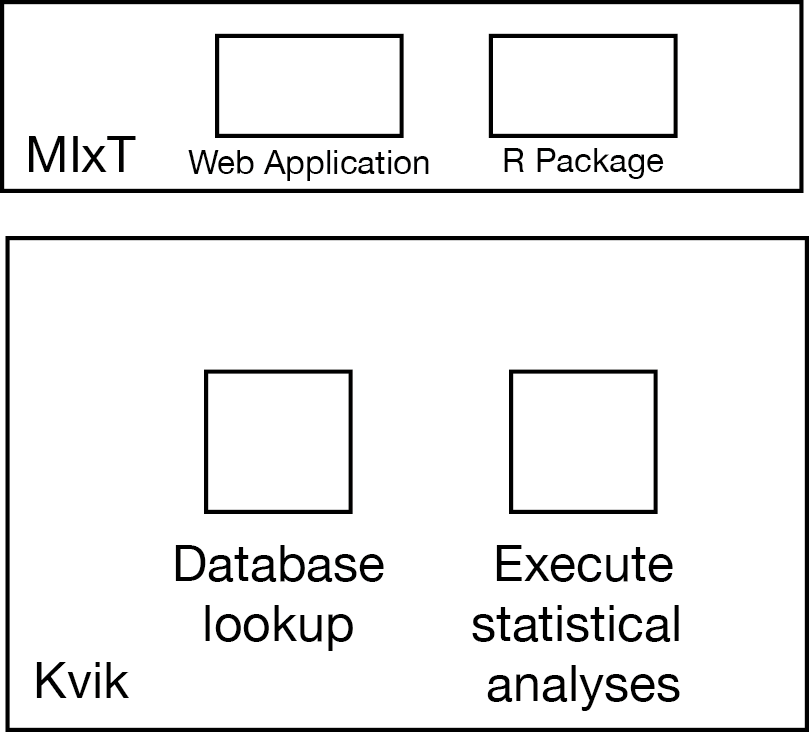
\includegraphics{figures/kvik-mixt.png}
\caption{An overview of the relationship between the MIxT application and Kvik.
MIxT contains a web application (online at \url{mixt-blood-tumor.bci.mcgill.ca})
and the R Package that provides analyses and data to the web application. Kvik
provides the services for running the statistical analyses from the R package,
and the database lookups found in the web application.} 
\label{kvik-mixt}
\end{figure} 

It is important to note that since the end applications interface directly with
R, developers can leverage this to produce dynamic visualizations. For example,
if an application uses a clustering method to color nodes in a graph, end-users
can tweak parameters that interactively change the node coloring in graph
visualization.
% LAB: hvordan?

% LAB: mangler beskrivelse av reference databases

% LAB: kan kuttes. Dette er motivasjon som skal være beksrevet tidligere
In Kvik we do not specify what programming language or set of tools to use to
build an application. We believe that by building an application as a set of
services that communicate over standard protocols, application developers can
choose the most suitable language, or framework, to build specialized
visualizations and user interfaces. 

\subsubsection*{Applications}

% LAB: Kort om hva en appliacation gjør og ikke gjør. Og hvor den kjøres.

\subsubsection*{Compute Service}
% LAB: Ikke motivert hvorfor det er en interface til R
% LAB: Ikke forklart hvordan en appliakasjons programmerer skal tenke på denne servicen. Dvs hva den brukes til og hva den tilbyr. Første paragraf hopper rett inn i interfacen.
% Hva er fordelene med å gjøre det i go?
The compute service in Kvik is built using a hybrid state pattern\cite{opencpu}.
% LAB: hva er hybrid state pattern?
We provide three main operations for interfacing with R:
Call, Get, and RPC. The Call operation is used to execute and run a function
from an R package. 
% LAB: Hvorfor kun en slik minimalistisk interface? Og ikke høyere nivå operasjoner, eller noe for å skjule R? (mener ikke at det er en god ide å gjøre det slik, men det bør sies hvorfor disse 3 er ett fornuftig valg)
% LAB: hvordan blir dette kjørt? i en tråd? ny process?
It takes as input an R package name, a function name, and
optional arguments. It returns a unique identifier that later can be used by the
Get operation to retrieve results. The Get operation is used to get results in
different output formats, e.g. JSON, CSV, PDF, or PNG. The RPC is just a
combination of a Call and a subsequent Get. 
% LAB: error handling?
% LAB: data access?
% LAB: initialization?

% LAB: Ikke nødvendigvis klart for leseren hva som er fordelene med en slik
% microservice. Eller hvorfor det blir enklere å utivkle apps vha denne.

% LAB: performance, scalability, & provenance?

% LAB: mangler detaljer om bruk av containers, hvordan funksjoner blir kjørt (ikke alle har oversikt over hvordan R fungerer), mulighet for flere concurrent funksjoner, multi-threading/processing/paralleisering, distribusjon/ replikering av servere, caching. 

\subsubsection*{Database Service} 
The database service provides an interface to biological databases for
retrieving meta-data on genes and processes. 
% LAB: mangler detaljer for interfacen
% LAB: provencance, performance, scalability
% LAB: Dette kan tas på slutten
We have currently packages for
interfacing with
E-utilities\footnote{\url{eutils.ncbi.nlm.nih.gov}},
MSigDB\footnote{\url{software.broadinstitute.org/gsea/msigdb}}, Hugo Gene
Nomenclature Committe (HGNC)\footnote{\url{genenames.org}}, and Kyoto Encyclopedia
of Genes and Genomes (KEGG)\footnote{\url{kegg.jp}}. 

TODO: Talk about licensing issues. 

% LAB: Dette er veldig overfladisk beskrevet. Hvordan bruker application
% programmerern den? Hvor lagres ting? Hva slags datastrukturer brukes? Hvor
% stor er cachen? Er den delt? Eviction policy? Antatt size på working set? Er
% den komprimert? etc
% LAB: flere ting: deling av cache mellom apps, mulighet for prefetch, hva skjer når service starter/stopper og hvor ofte gjøres det?
The database service uses a caching mechanism to reduce the load on the online
databases. It will also speed up subsequent queries for a cached object, since
the query can be served out of cache and not having to be fetched from a remote
database. 
% LAB: ingen persistance? som ikke er bra for provenance.
We allow application developers to specify the cache eviction policy,
but on default the database service does not evict anything from its cache
before the service is restarted. This can be modified by the application
developer. 

% LAB: fordel av å bruke den; hvorfor det gjør livet enklere...

% LAB: savner en beskrivelse (del kapittel) av deployment og andre ting som har med management av disse services og apps

\subsection*{Implementation}
In ths section we describe the implementation details in Kvik its
microservices.

Kvik is implemented as a collection of Go packages required to build services
that can integrate statistical
software in a data exploration and provide an interface to up-to-date biological
databases. We chose the Go programming language because of its performance, ease
of development, and simple deployment. 
To integrate R we provide two packages \emph{gopencpu} and
\emph{r}, that interface with OpenCPU and Kvik R servers respectively. To
interface with biological databases we provide the packages \emph{eutils},
\emph{gsea}, \emph{genenames}, and \emph{kegg} that interface with E-utils,
MsigDB, HGNC and KEGG respectively.
In addition to these packages we provide Docker images that implement the
two required microservices. 

Both the compute and the databases service in Kvik builds on the standard
\emph{http} library in Go. On start the compute service 
launches a user-defined number of R sessions that execute analyses on demand.
This allows for parallel execution of analyses. We provide a simple FIFO queue
for queuing of requests. The compute service also provides the opportunity for users to
cache analysis results to speed up subsequent calls. The database service use
the \emph{gocache}\footnote{\url{github.com/fjukstad/gocache}} package to cache
any query to an online database.

% LAB: Litt usikker på om dette hører til i Results eller Methods
% \subsection*{Applications}
% Stress.
% Pathways.
% MIxT .
% Command line-man. 
% 
% % LAB: kort beskrivelse av hva alle apps gjør
% 
% % LAB: Figur som viser hva som er felles og ulikt for alle appene. Her bør noe
% % være likt ellers har vi bare 3-4 applikasjoner :)
% 
% % LAB: mer detaljert beskrivelse av hvordan hver app er implementert med Kvik
% 
% 
